\documentclass[11pt]{article}
%
\usepackage{basic}
\newcommand{\tinydots}{\hbox to 1em{.\hss.\hss.}}
% 
\newcommand{\anne}[1]{{\color{pink!50!blue}Anne:~#1}}
\newcommand{\joel}[1]{{\color{red!50!orange}Joel:~#1}}
\newcommand{\todo}[1]{{\color{red!50!white}\textbf{#1}}} % TODO
%
\title{Case study: weight $\alpha_1 + 2\alpha_2 + \alpha_3$ in type $A_3$}
\author{Elie, Anne, Joel}
\begin{document}
\maketitle
%
We would like to deform the map $\barD : \CC[N]\to \CC[\treg]$ such that \todo{what}. 
To this end, we sample/compare candidates for quantum and asymptotic versions of $\barD$ on elements of the MV basis of weight $\nu = (1,2,1) = \alpha_1 + 2\alpha_2 + \alpha_3$. The dimension of $\CC[N]_{-\nu}$ is $\kpf(\nu) = 5$. The five \todo{partitions} of $\nu$ are:
\begin{enumerate}
    \item $(\alpha_1 + \alpha_2) + (\alpha_2) + (\alpha_3)$
    \item $(\alpha_1 + \alpha_2 + \alpha_3) + (\alpha_2)$
    \item $(\alpha_1 + \alpha_2) + (\alpha_2 + \alpha_3)$
    \item $(\alpha_1) + (\alpha_2) + (\alpha_2 + \alpha_3)$
    \item $(\alpha_1) + 2(\alpha_2) + (\alpha_3)$
\end{enumerate}
% 
Fix the order $3 < 2 < 1$ on $I$ and fix the \todo{compatible} reduced expression $\uvi = (1,2,3,1,2,1)$ for $w_0\in W$. 

\anne{Verify that this is indeed the order we want!} 

With respect to these choices, we can replace the above list of partitions by \todo{Lusztig data}:  
\begin{enumerate}
    \item $(0,1,0,1,0,1)$
    \item $(0,0,1,1,0,0)$
    \item $(0,1,0,0,1,0)$
    \item $(1,0,0,1,1,0)$
    \item $(1,0,0,2,0,1)$
\end{enumerate}
Nb.\ There are exactly five Lusztig data of weight $\nu$.

\anne{We will also record this list using \todo{Lyndon words}. In what follows we write words using redundant dots to exaggerate the constituent \todo{good} \todo{root} words?}

For each of the above (triples of) combinatorial data (partition, Lusztig datum, Lyndon word) we record the corresponding MV cycle, its polytope, its multidegree, its (zeroth) equivariant multiplicity, and its (multigraded) Hilbert series. 
% There are five MV cycles $\irr\overline{S^0\cap T^\nu}$ 

We also record the irreducible character and residual $\barD$ of the corresponding simple module for the KLR algebra. 
% The KLR algebra is R^0_\nu? 

% \begin{question}
\anne{Does there exist some natural order on Lusztig data? aka, on Kostant partitions?}
% \end{question}

For the time being we use two equivalent conventions:
\begin{enumerate}
    \item {\color{red}The word for the positive root $\alpha_i + \cdots + \alpha_j$ is $i\,i+1\,\cdots\,j$ i.e.\ increasing wrt $1 < 2 < 3$, and root words are concatenated in decreasing order} (Mine)
    \item {\color{blue}The word for the positive root $\alpha_i + \cdots + \alpha_j$ is $j\,j-1\,\cdots\,i$ i.e.\ decreasing wrt $1 < 2 < 3$, and root words are concatenated in increasing order} (Elie's)
\end{enumerate}
\section*{The data}
\begin{description}
    \item[{\bf 1.} $n_\bullet = (0,1,0,1,0,1)$:] 
    % $; $\lambda = (4,3,1,0)$ and $\mu = (3,2,2,1)$ 
    \[
        \underline{w}[n_\bullet] ={\color{red}3.2.12} = {\color{blue}21.2.3} \qquad \lambda = (4,3,1,0) \ge \mu = (3,2,2,1)
    \]
% 
% \begin{figure}[ht!]
% \begin{center}
    {\small$$
    \begin{gathered}
        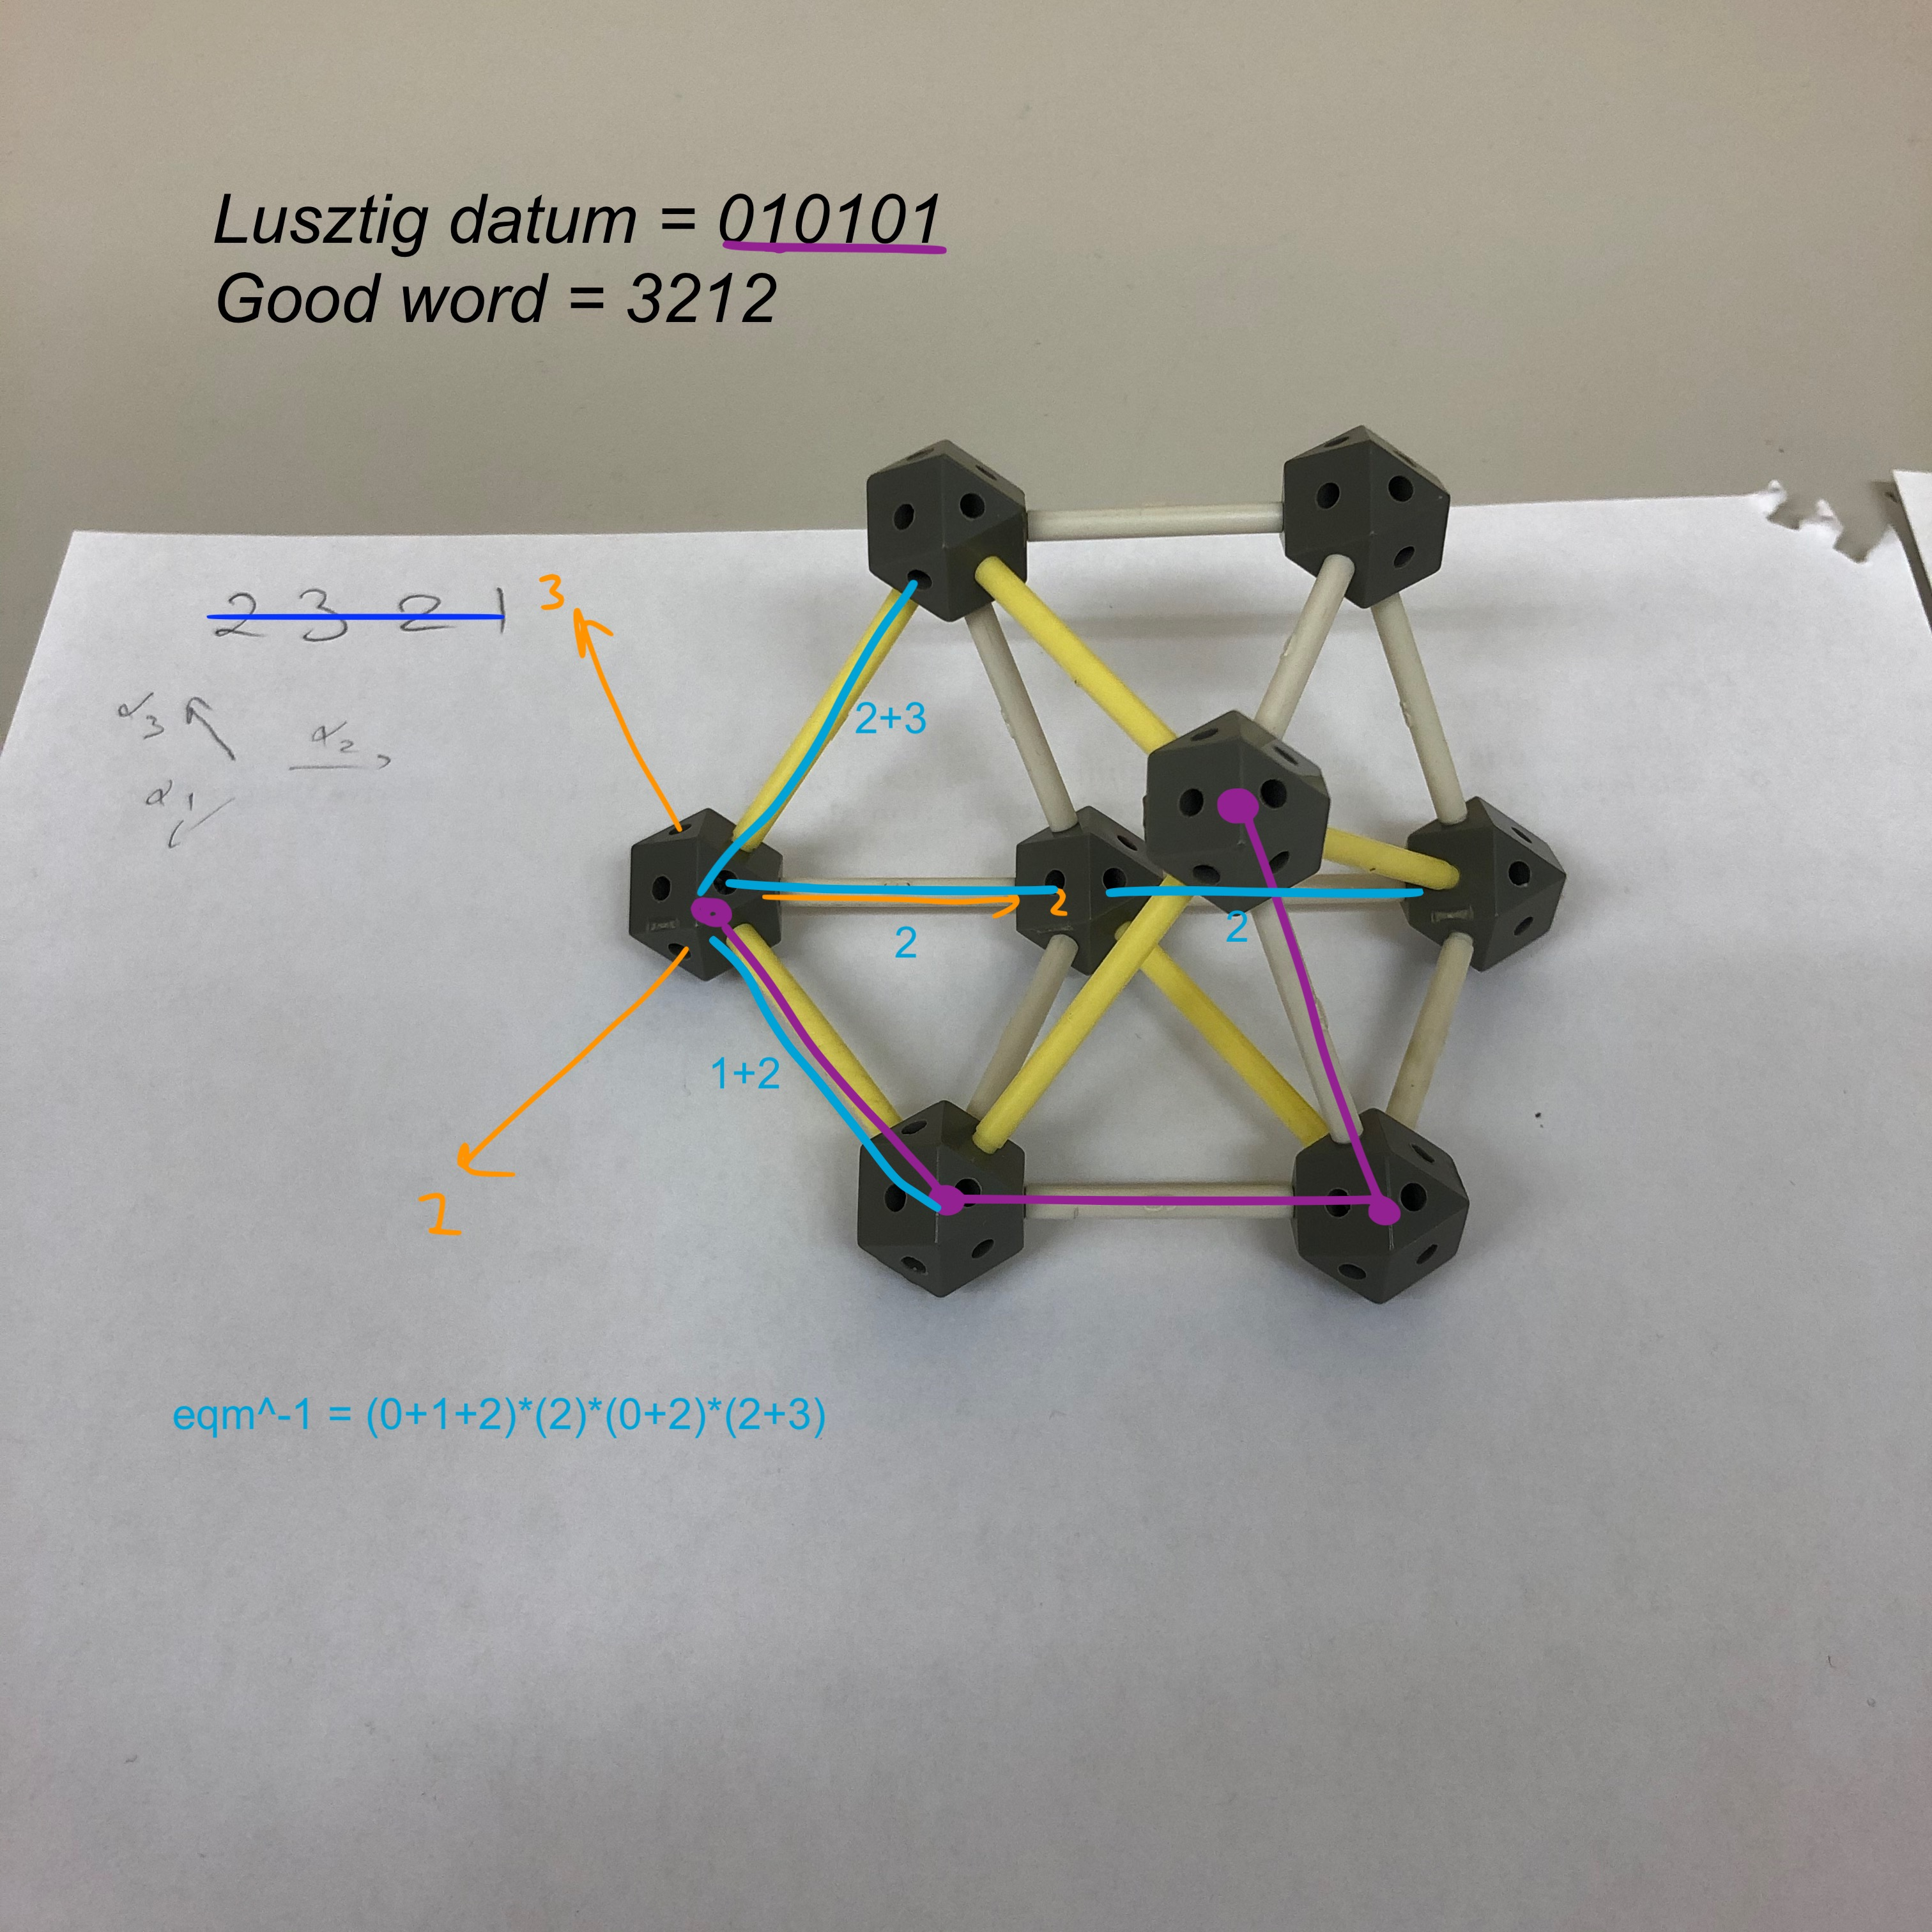
\includegraphics[height=100px]{img/3212.jpeg} 
    \end{gathered}= \Conv(\alpha_2, \alpha_1 + \alpha_2,\alpha_1 + 2\alpha_2, 2\alpha_2, 2\alpha_2+\alpha_3,\alpha_2+\alpha_3,\nu) 
    $$}
% \end{center}
% \caption{Lyndon word 3212}
% \end{figure}

From \todo{its tableau} 
\[
    \tau = \young(1113,223,4)
\]
we find the ideal of the corresponding MV cycle in $\CC[a_1..a_9]$ where $a_i$ are coordinates on $\TT_\mu\cap\n$ and $\Gr_\mu\cap S^\mu_-$ which are related by the MVy isomorphism
{\small$$\left[\begin{BMAT}{ccc:cc:cc:c}{ccc:cc:cc:c}
    0&1&0&0&0&0&0&0\\
    0&0&1&0&0&0&0&0\\
    0&0&0&{a}_{1}&{a}_{2}&{a}_{3}&{a}_{4}&{a}_{5}\\
    0&0&0&0&1&0&0&0\\
    0&0&0&0&0&{a}_{6}&{a}_{7}&{a}_{8}\\
    0&0&0&0&0&0&1&0\\
    0&0&0&0&0&0&0&{a}_{9}\\
    0&0&0&0&0&0&0&0\end{BMAT}\right]
    \mapsto \begin{bmatrix}
        t^3 \\
        -a_1 -a_2t & t^2 \\
        -a_3 -a_4t & -a_6 - a_7 t & t^2 \\
        -a_5 & -a_8 & -a_9 & t 
    \end{bmatrix}
$$}
The ideal is found by imposing rank conditions on (principal submatrices of) $X\in\TT_\mu\cap\n$ coming from the shapes of the nested sequence of subtableaux of $\tau$
$$
\young(111,2)\subset\young(111,22)\subset\young(111,223)\subset\young(1113,223) \subset \tau 
$$
It is $I = \left({a}_{1},{a}_{2},{a}_{3},a_9,a_5\right)$. 
As an aside, we also check the assignment $\tau\mapsto w(\tau)$ that plays a key role in our conjectural recursive description of $I$. Here $w(\tau) = {123\atop 213}$ and indeed the second entry in the last column of the matrix above is free. Recall that the total number of free entries expected is $4 - \text{row}(4)$. 
% Errors: had {a}_{6},{a}_{4}
% 

The multidegree of $I$ is 
% $$
% \mdeg I = (\alpha_1)(\alpha_1 + \hbar) (\alpha_1 + \alpha_2) (\alpha_1 + \alpha_2 + \alpha_3) (\alpha_2 )
% $$
% and verify using M2 to find that actually we made a booboo, it should be 
% $$
% \mdeg I = (\alpha_1)(\alpha_1 + \hbar) (\alpha_1 + \alpha_2) (\alpha_1 + \alpha_2 + \hbar) (\alpha_2)
% $$
\[
\mdeg I = \left(\alpha_{1}+{\alpha}_{2}\right)\left({\alpha}_{3}+{\alpha}_{1}+\alpha_2\right)\left(\hbar+{\alpha}_{1}\right)\left({\alpha}_{1}{\alpha}_{3}\right)    
\]
The equivariant multiplicity of $I$ at zero is got by normalizing the multidegree by dividing by the multidegree of zero in the ambient affine space $\TT_\mu\cap\n$ (i.e.\ the multidegree of the ideal of zero). It is
$$
% boo boo persisting: \varepsilon^{T\times\CC^\times}_0(I) = \frac{1}{(\alpha_1 + \alpha_2 + \hbar)(\alpha_2 + \hbar) (\alpha_2 + \alpha_3) (\alpha_3 )}
% \varepsilon^{T\times\CC^\times}_0(I) = \frac{1}{(\alpha_1 + \alpha_2 + \alpha_3)(\alpha_2 + \hbar) (\alpha_2 + \alpha_3) (\alpha_3 )}
\varepsilon^{T\times\CC^\times}_0(I) = \frac{1}{(\alpha_1 + \alpha_2 + \hbar)(\alpha_2)(\alpha_2+\hbar)(\alpha_2 + \alpha_3)}
$$

Using Macaulay2 we find that $I$ has $T\times\CC^\times$-graded Hilbert series
% $$
% \frac{1}{\left(1-{T}_{0}{T}_{1}{T}_{2}\right)\left(1-{T}_{1}{T}_{2}\right
%     )\left(1-{T}_{1}{T}_{3}\right)\left(1-{T}_{2}\right)}
% $$
\[
    \frac{1}{\left(1-{T}_{0}{T}_{1}{T}_{3}\right)\left(1-{T}_{1}{T}_{2}\right)\left(1-{T}_{1}\right)\left(1-{T}_{1}{T}_{3}\right)}    
\]
\anne{The $T$'s here are formal variables keeping track of the weights of the torus $\times$ loop rotation action, as multiplicative weights, i.e.\ characters. 
Does $q$ also do this? I would like to \todo{justify} rewriting this Hilbert series as 
\[
    % \frac{1}{(1 - q^{\alpha_1 + \alpha_2 + \hbar})(1-q^{\alpha_2 + \alpha_3})(1-q^{\alpha_2})(1-q^{\alpha_2 + \hbar})}    
    \frac{1}{(1 - e^{\alpha_1 + \alpha_2 + \hbar})(1-e^{\alpha_2 + \alpha_3})(1-e^{\alpha_2})(1-e^{\alpha_2 + \hbar})}    
\]
}

\joel{What are these $T$s? And what do you mean here by $ q^\alpha$? If you just mean $ \alpha$ but in multiplicative notation, maybe it would be better to write $ e^\alpha$ to avoid confusion with the $ q $ occurring later in Elie's $D_q$.}

\anne{Yes! Definitely: $e^\alpha$ is a more appropriate substitution. Another thing we should check is if the coincidence we are observing in this case persists in higher rank. The guess is that MV $\neq$ dual canonical so we should actually witness the $q=1$ substition fail to recover $\varepsilon$ at some point.}

Jon Brundan's program outputs dual canonical basis elements.
Using Jon Brundan's program, the irreducible character of the simple KLR module $L$ with the given Lusztig datum is 
% IC[4] = 
\[
    \ch L = [1|2|3|2]+(q+q^{-1})[1|3|2|2]+(q+q^{-1})[3|1|2|2]+[3|2|1|2]
\]
\anne{Now, I am not sure whether these words should be read using the red convention or the blue. But, according to Joel, (according to Elie,) $\barD(L)$  is obtained from $\ch L$ by replacing each $\underline{w}[i_1..i_4]$ by 
$$\barD_{\underline{w}[i_1..i_4]}:= \frac 1 {\alpha_{i_1}(\alpha_{i_1} + \alpha_{i_2})(\alpha_{i_1} + \alpha_{i_2} + \alpha_{i_3})(\alpha_{i_1}+\alpha_{i_2} + \alpha_{i_3}+\alpha_{i_4})}$$ and summing. In fact, the thing that seems to work is reading these guys in reverse---Elie's convention??---i.e.\ replacing $\underline{w}[i_1..i_4]$ by 
$$\barD_{\underline{w}[i_1..i_4]}:= \frac 1 {\alpha_{i_4}(\alpha_{i_3} + \alpha_{i_4})(\alpha_{i_2} + \alpha_{i_3} + \alpha_{i_4})(\alpha_{i_1}+\alpha_{i_2} + \alpha_{i_3}+\alpha_{i_4})}$$ 
In this case, we find % something ghastly
{\tiny
$$
\barD (L) =
% \hspace*{-5.5cm}
\begin{aligned}{a}_{1}^{2}{a}_{2}q^{2}+5\,{a}_{1}{a}_{2}^{2}q^{2}+4\,{a}_{2}^{3}q^{2}+{a}_{1}^{2}{a}_{3}q^{2}+6\,{a}_{1}{a}_{2}{a}_{3}q^{2}\\
    +5\,{a}_{2}^{2}{a}_{3}q^{2}+{a}_{1}{a}_{3}^{2}q^{2}+{a}_{2}{a}_{3}^{2}q^{2}+2\,{a}_{1}^{2}{a}_{2}q+6\,{a}_{1}{a}_{2}^{2}q+8\,{a}_{2}^{3}q \\ 
    \frac{+6\,{a}_{2}^{2}{a}_{3}q+2\,{a}_{2}{a}_{3}^{2}q+{a}_{1}^{2}{a}_{2}+5\,{a}_{1}{a}_{2}^{2}+4\,{a}_{2}^{3}+{a}_{1}^{2}{a}_{3}+6\,{a}_{1}{a}_{2}{a}_{3}+5\,{a}_{2}^{2}{a}_{3}+{a}_{1}{a}_{3}^{2}+{a}_{2}{a}_{3}^{2}}{\left(q\right)\left({{a}_{2}}\right)^{2}\left({a}_{2}+{a}_{3}\right)\left(2\,{a}_{2}+{a}_{3}\right)\left({a}_{1}+{a}_{2}\right)\left({a}_{1}+2\,{a}_{2}\right)\left({a}_{1}+2\,{a}_{2}+{a}_{3}\right)\left(2\right)}
\end{aligned}
$$}
That's a big numerator---M2 doesn't want to (really can't?) simplify it. 
Evaluating at $q = 1$ we recover
$$\frac{1}{\left({{a}_{2}}\right)^{2}\left({a}_{2}+{a}_{3}\right)\left({a
      }_{1}+{a}_{2}\right)}$$
as desired! I'll take this approach in all subsequent calculations, sans annotations. 

\todo{Warning!} That's $\varepsilon^{T\times\CC^\times}(I)\big|_{\hbar = 0} = \varepsilon^{T}(I)$. How do we forget less and recover $\varepsilon^{T\times\CC^\times}(I)$ instead? No clear route from $q$-graded character to $\hbar$-equivariant multiplicity, yet!
} 
\item[{\bf 2.} $n_\bullet = (0,0,1,1,0,0)$:] 
% $\lambda = (3,2,0,0)$ and $\mu = (2,1,1,1)$ \hfill 
\[
    \underline{w}[n_\bullet] = {\color{red} 2.123} = {\color{blue} 2.321} \qquad  \lambda = (3,2,0,0) \ge \mu = (2,1,1,1)
\]
\[
    \begin{gathered}
        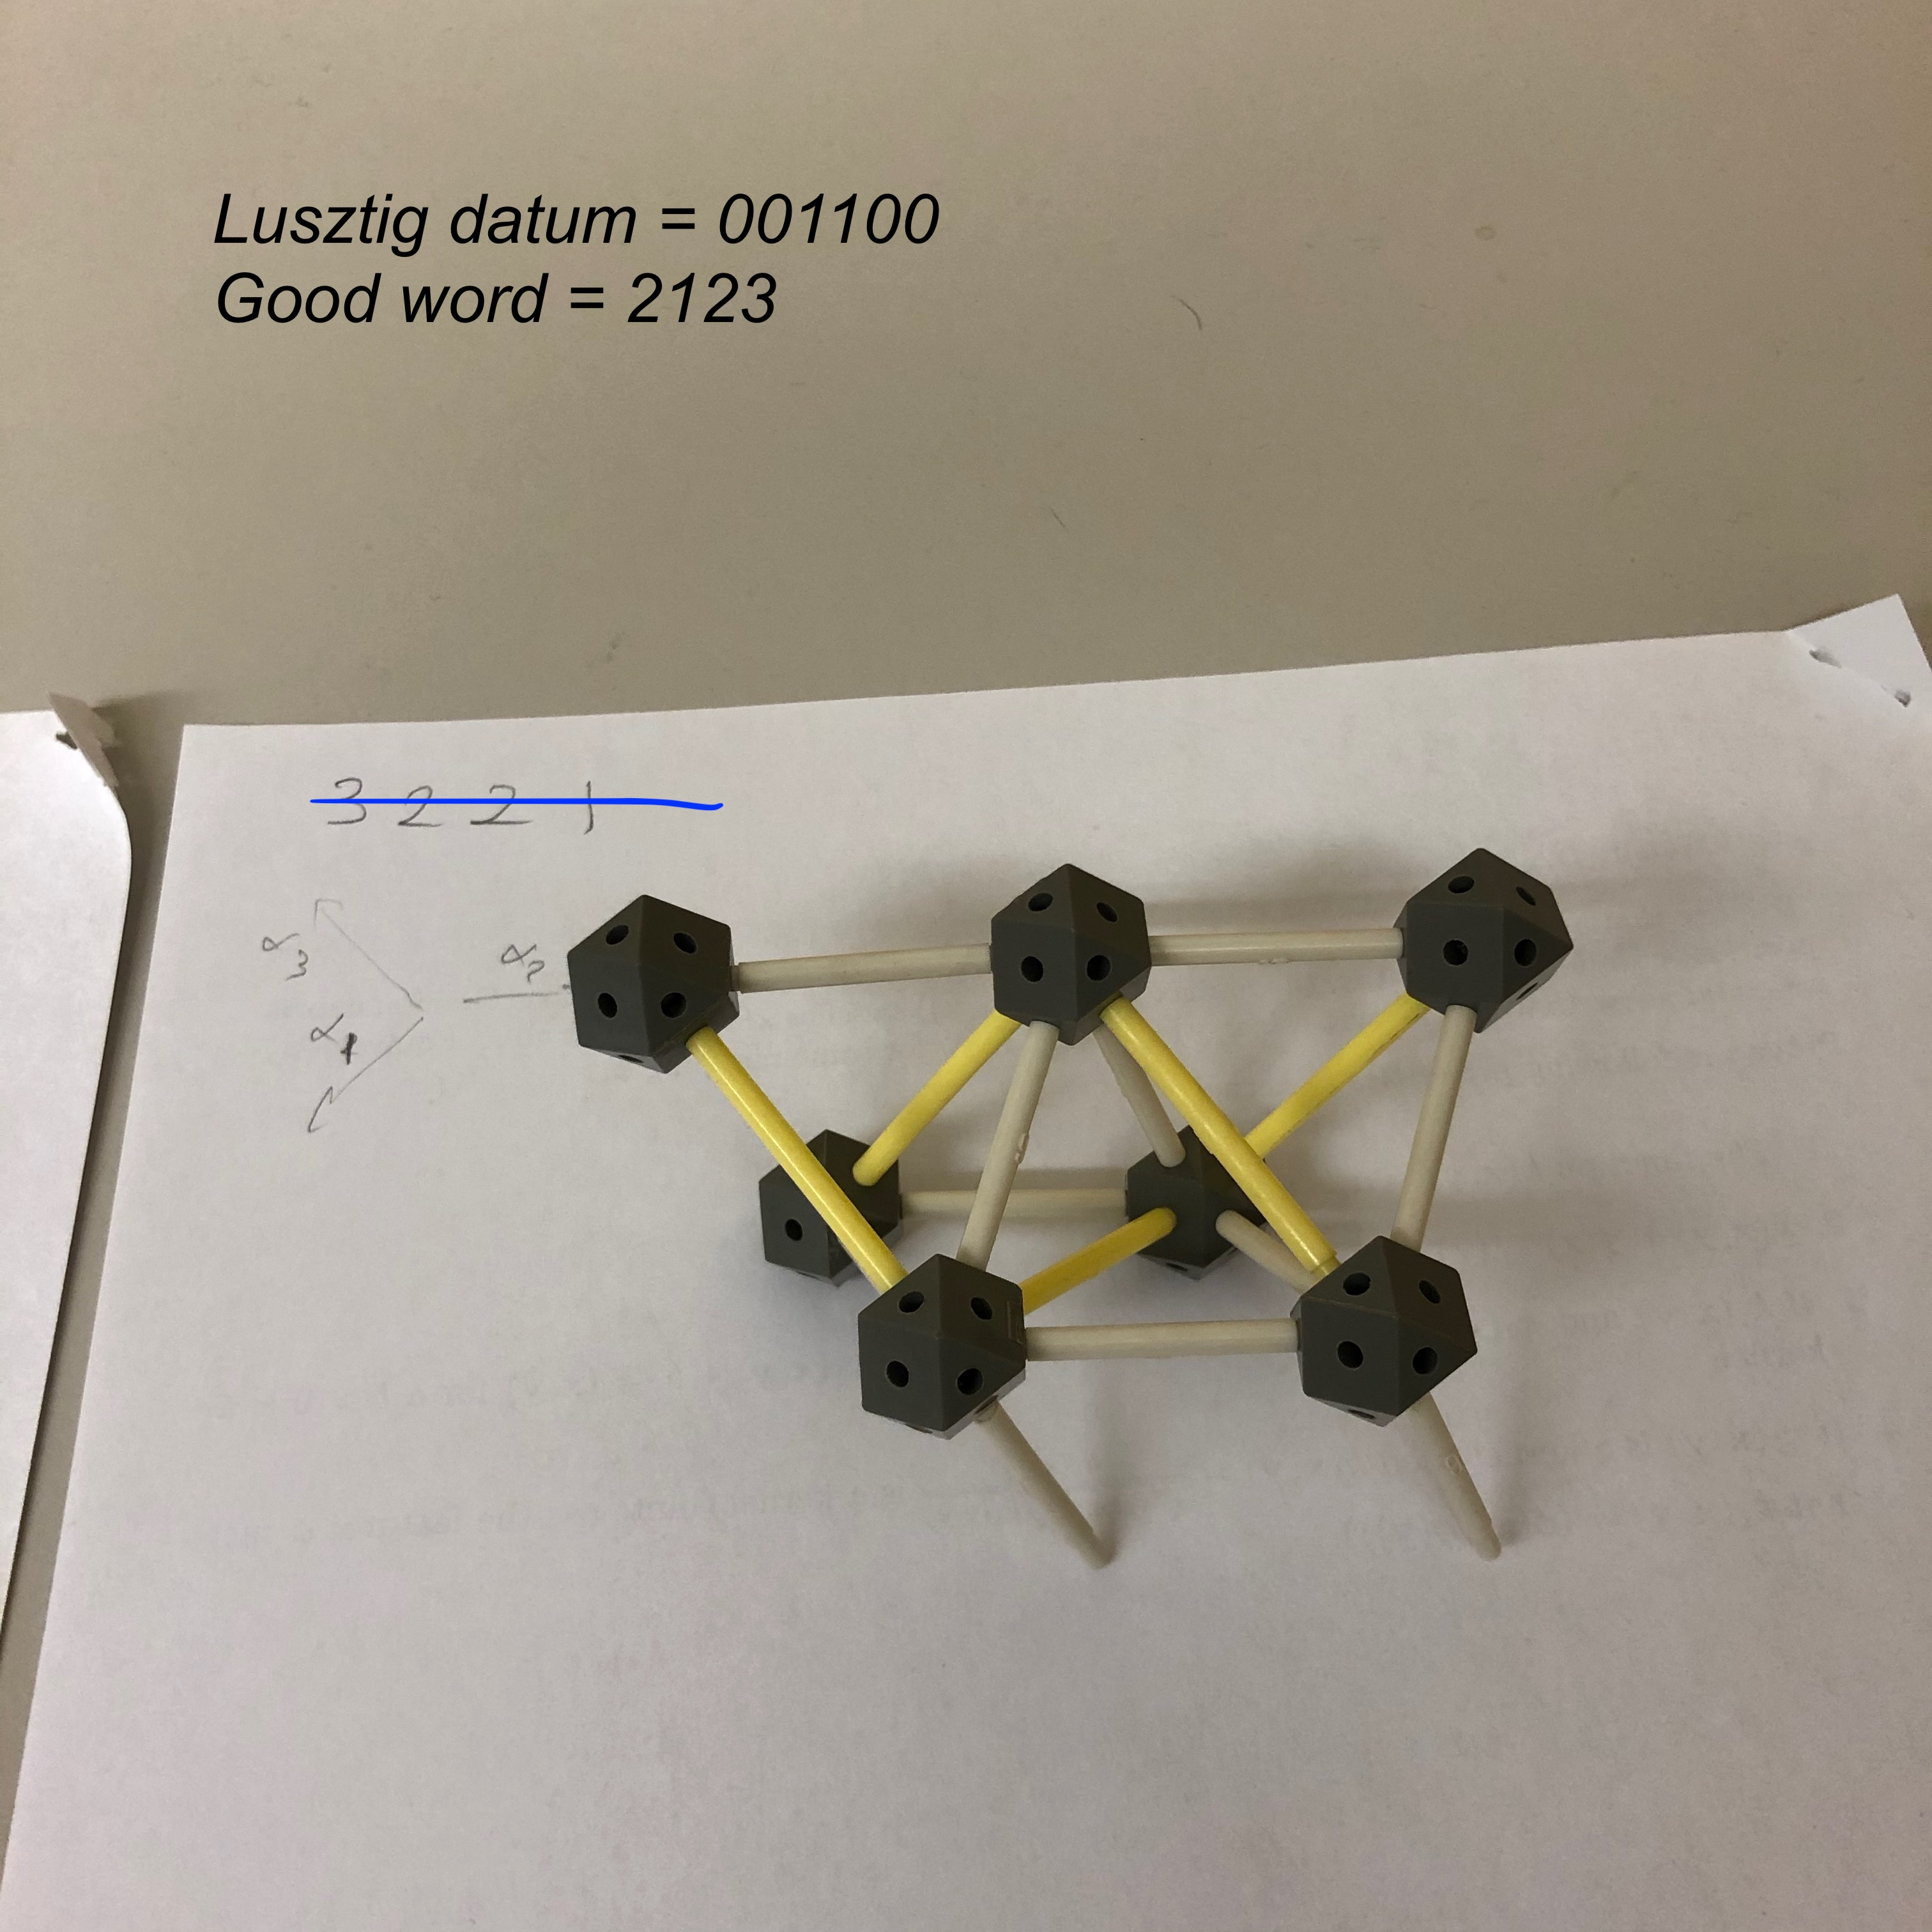
\includegraphics[height=100px]{img/2123.jpeg}
    \end{gathered} = \Conv(\alpha_2,\alpha_2 + \alpha_3,2\alpha_2 + \alpha_3,\alpha_3,\alpha_1 + \alpha_2 + \alpha_3,\nu)
\]
From its tableau 
$$
\young(114,23)
$$
we find the ideal of the corresponding MV cycle in $\CC[a_1..a_6]$ by imposing rank conditions on matrices of the form below (left) 
$$\begin{pmatrix}
    0&1&0&0&0\\
    0&0&{a}_{1}&{a}_{2}&{a}_{3}\\
    0&0&0&{a}_{4}&{a}_{5}\\
    0&0&0&0&{a}_{6}\\
    0&0&0&0&0\end{pmatrix}\mapsto \begin{pmatrix}
        t^2 \\
        -a_1 & t \\
        -a_2 & -a_4 & t \\
        -a_3 & -a_5 & -a_6 & t 
    \end{pmatrix}$$
coming from the shapes of the nested sequence of subtableaux of $\tau$
$$
\young(11,2)\subset\young(11,23)
$$
so $I = (a_1,a_2)$.
Note that $w(\tau) = {123\atop 231}$, although in this case, all three entries in the last column of the matrix above are free, so the order is redundant? 
The multidegree of $I$ is
$$
\mdeg I = (\alpha_1) (\alpha_1 + \alpha_2)
$$
% double check in M2 which gives $\left({T}_{0}+{T}_{1}\right)\left({T}_{0}\right)$
So its equivariant multiplicity (at zero) is   
$$
\varepsilon^{T\times\CC^\times}_0(I) = \frac{1}{(\alpha_1 + \alpha_2 + \alpha_3)(\alpha_2)(\alpha_2 + \alpha_3)(\alpha_3)}
$$
Using M2 we find that $I$ has Hilbert series
$$\frac{1}{\left(1-{T}_{0}{T}_{1}{T}_{2}\right)\left(1-{T}_{1}{T}_{2}\right)\left(1-{T}_{2}\right)\left(1-{T}_{1}\right)}$$
% 
Using Jon Brundan's program, the character of the corresponding simple $L$ is 
% IC[1] = 
\[
    \ch L = (q+q^{-1})[1|2|2|3]+[1|2|3|2]+[2|1|2|3]   
\]
so 
{\tiny
\[
\barD (L) = 
\frac{{a}_{1}{a}_{2}q^{2}+{a}_{2}^{2}q^{2}+{a}_{2}{a}_{3}q^{2}+2\,{a}_{2}^{2}q+{a}_{1}{a}_{3}q+2\,{a}_{2}{a}_{3}q+{a}_{3}^{2}q+{a}_{1}{a}_{2}+{a}_{2}^{2}+{a}_{2}{a}_{3}}{\left(q\right)\left({a}_{3}\right)\left({a}_{2}\right)\left({a}_{2}+{a}_{3}\right)\left(2\,{a}_{2}+{a}_{3}\right)\left({a}_{1}+{a}_{2}+{a}_{3}\right)\left({a}_{1}+2\,{a}_{2}+{a}_{3}\right)}  
\]}
and evaluating at $q = 1$ we recover 
\[
    \frac{1}{\left({a}_{3}\right)\left({a}_{2}\right)\left({a}_{2}+{a}_{3}\right)\left({a}_{1}+{a}_{2}+{a}_{3}\right)}
\]
    % 
\item[{\bf 3.} $n_\bullet = (0,1,0,0,1,0)$:] 
% $\lambda = (2,2,0,0)$ and $\mu = (1,1,1,1)$ \hfill 
\[
\underline{w}[n_\bullet] =  {\color{red}23.12} = {\color{blue}21.32} \qquad \lambda = (2,2,0,0) \ge \mu = (1,1,1,1)  
\]
\[
    \begin{gathered}
        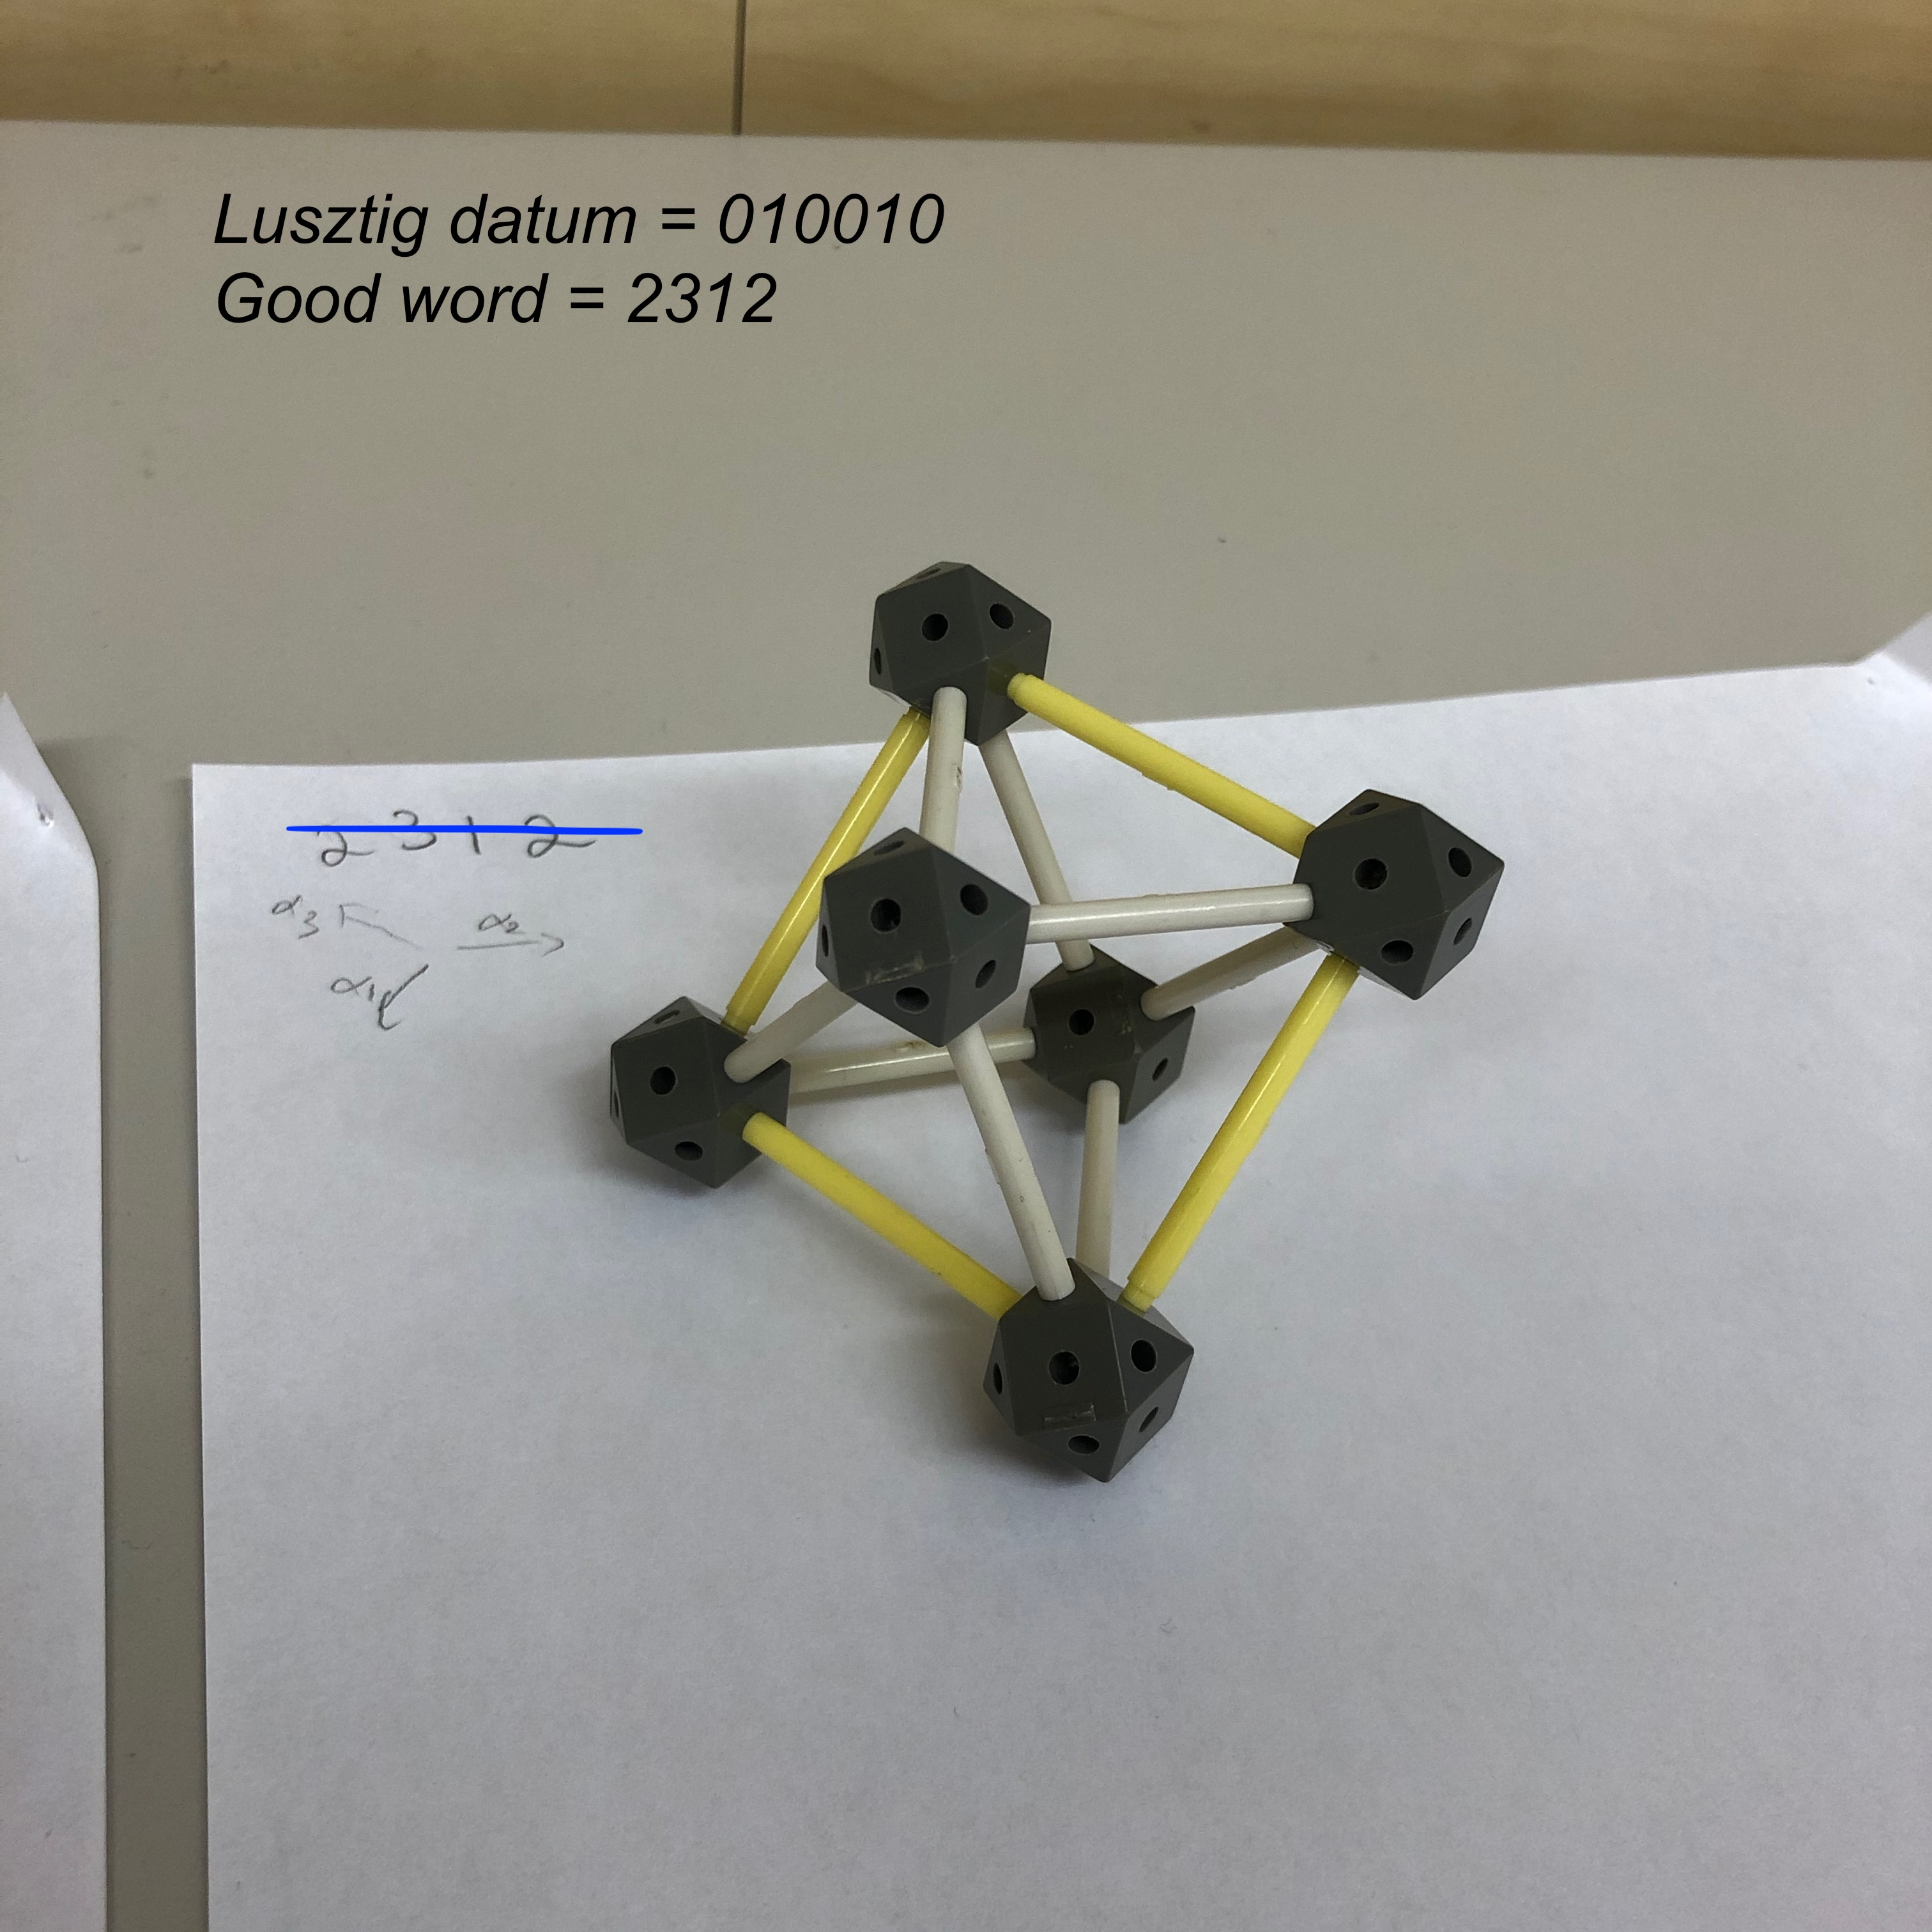
\includegraphics[height=100px]{img/2312.jpeg}
    \end{gathered} = \Conv(2, 1 + 2, 1 + 2 + 3, 2 + 3, \nu) 
\]
% 
From its tableau 
$$
\young(13,24)
$$
we find the ideal of the corresponding MV cycle in $\CC[a_1..a_6]$ by imposing rank conditions on matrices of the form below (left)
$$\begin{pmatrix}
    0&{a}_{1}&{a}_{2}&{a}_{3}\\
    0&0&{a}_{4}&{a}_{5}\\
    0&0&0&{a}_{6}\\
    0&0&0&0\end{pmatrix}\mapsto \begin{pmatrix}
        t \\
        -a_1 & t \\
        -a_2 & -a_4 & t \\
        -a_3 & -a_5 & -a_6 & t
\end{pmatrix}$$
coming from shapes of the nested sequence of subtableaux of $\tau$
\[
\young(1,2)\subset\young(13,2)
\]
so $I = (a_1,a_6)$. Note that $w(\tau) = {123\atop 213}$ and the second and first entries in the last column of the matrix above are free.
Its multidegree is
$$
\mdeg I = (\alpha_1) (\alpha_3)
$$
So its equivariant multiplicity (at zero) is  
$$
\varepsilon^{T\times\CC^\times}_0(I) = \frac{1}{(\alpha_1 + \alpha_2)(\alpha_1 + \alpha_2 + \alpha_3)(\alpha_2)(\alpha_2 + \alpha_3)}
$$
Using M2 we find that $I$ has Hilbert series 
\[
    TODO 
\]
Using JB, the character of the corresponding simple $L$ is 
% IC[2] 
\[
    \ch L = [2|1|3|2]+[2|3|1|2]
\]
Note that it is symmetric and that there are no $q$'s. 
\[
    \barD(L) = \frac 1 {(a_2) (a_2 + a_3) (a_1 + a_2) (a_1 + a_2 + a_3)}
\]
\item[{\bf 4.} $n_\bullet = (1,0,0,1,1,0)$:] 
% $\lambda = (2,2,0,0)$ and $\mu = (1,1,1,1)$ \hfill 
\[
\underline{w}[n_\bullet] = {\color{red}23.2.1} = {\color{blue}1.2.32} \qquad \lambda = (2,2,0,0) \ge \mu = (1,1,1,1)
\]
\[
\begin{gathered}
    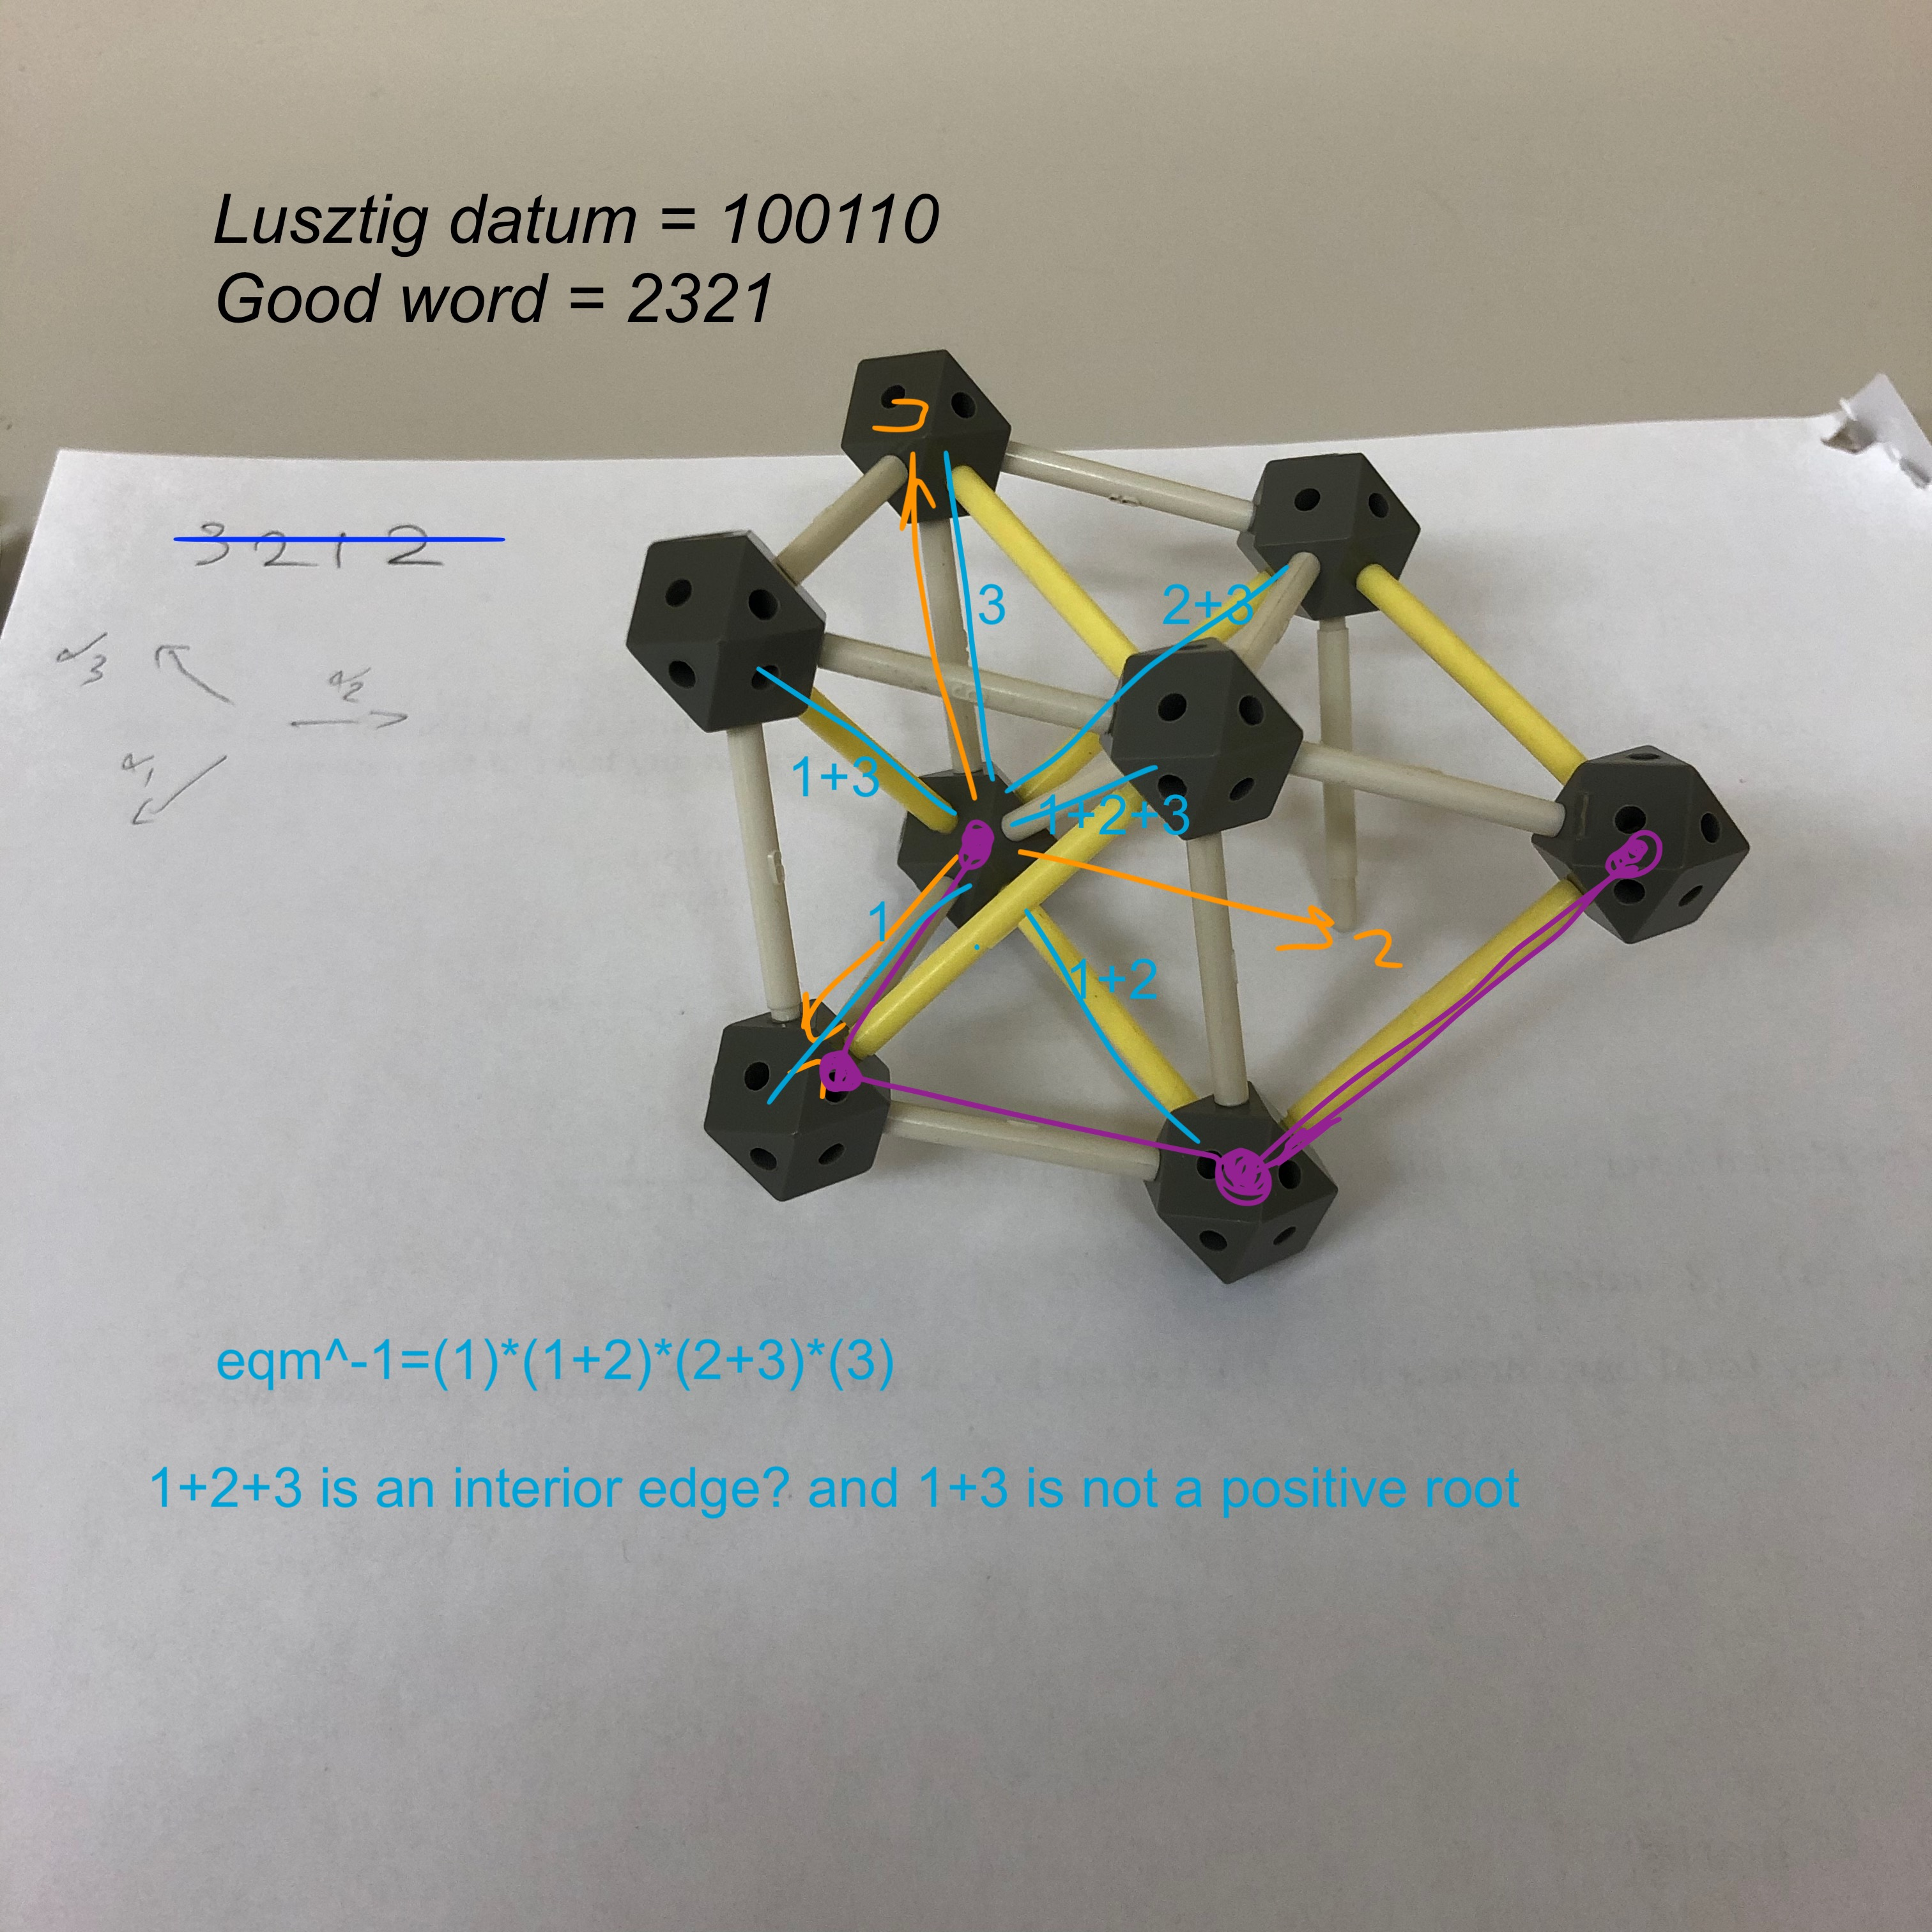
\includegraphics[height=100px]{img/2321.jpeg}
\end{gathered}
    = \Conv(1, 1 + 2, 1 + 2 + 3, 1 + 3, 3, 2 + 3, \nu)
\]
From its tableau 
$$\young(12,34)$$
we find the ideal of the corresponding MV cycle in \(\CC[a_1..a_6]\) by imposing rank conditions on matrices of the form below (left) 
$$\begin{pmatrix}
0&{a}_{1}&{a}_{2}&{a}_{3}\\
0&0&{a}_{4}&{a}_{5}\\
0&0&0&{a}_{6}\\
0&0&0&0\end{pmatrix}\mapsto \begin{pmatrix}
    t \\
    -a_1 & t \\
    -a_2 & -a_4 & t \\
    -a_3 & -a_5 & -a_6 & t
\end{pmatrix}$$
coming from shapes of the nested sequence of subtableaux of $\tau$ 
\[
    \young(12)\subset\young(12,3)
\]
so $I = \left({a}_{4},{a}_{1}{a}_{5}+{a}_{2}{a}_{6}\right)$. Note that $w(\tau) = {123\atop 132}$ and the first and third entries in the last column of the matrix above are free.
Its multidegree is 
$$
\mdeg I = (\alpha_2) (\alpha_1 + \alpha_2 + \alpha_3)
$$
So its equivariant multiplicity (at zero) is  
$$
\varepsilon^{T\times\CC^\times}_0(I) = \frac{1}{(\alpha_1)(\alpha_1 + \alpha_2)(\alpha_2 + \alpha_3)(\alpha_3)}
$$
Using M2 we find that $I$ has Hilbert series 
\[
    \frac{1}{\left(1-{T}_{1}{T}_{2}\right)\left(1-{T}_{0}{T}_{1}\right)\left(1-{T}_{2}\right)\left(1-{T}_{0}\right)}
\]
Using JB, the character of the corresponding simple $L$ is 
% IC[3] = 
\[
\ch L = [2|1|2|3]+(q+q^{-1})[2|2|1|3]+(q+q^{-1})[2|2|3|1]+[2|3|2|1]    
\]
So 
{\small \[
\barD (L) =     
\frac{{a}_{1}{a}_{2}q^{2}+{a}_{2}^{2}q^{2}+{a}_{1}{a}_{3}q^{2}+{a}_{2}{a}_{3}q^{2}+{a}_{1}^{2}q+{a}_{1}{a}_{2}q+{a}_{2}{a}_{3}q+{a}_{3}^{2}q+{a}_{1}{a}_{2}+{a}_{2}^{2}+{a}_{1}{a}_{3}+{a}_{2}{a}_{3}}{\left(q\right)\left({a}_{3}\right)\left({a}_{2}+{a}_{3}\right)\left({a}_{1}\right)\left({a}_{1}+{a}_{2}\right)\left({a}_{1}+{a}_{2}+{a}_{3}\right)\left({a}_{1}+2\,{a}_{2}+{a}_{3}\right)}
\]}
and evaluating at $q = 1$ we recover 
\[
    \frac{1}{\left({a}_{3}\right)\left({a}_{2}+{a}_{3}\right)\left({a}_{1}\right)\left({a}_{1}+{a}_{2}\right)}
\]
% Finally... 
\item[{\bf 5.} $n_\bullet = (1,0,0,2,0,1)$:] 
% $\lambda = (3,3,1,0)$ and $\mu = (2,2,2,1)$ \hfill 
\[
    \underline{w}[n_\bullet] = {\color{red} 3.2.2.1} = {\color{blue} 1.2.2.3} \qquad \lambda = (3,3,1,0) \ge \mu = (2,2,2,1)
\]
\[
\begin{gathered}
    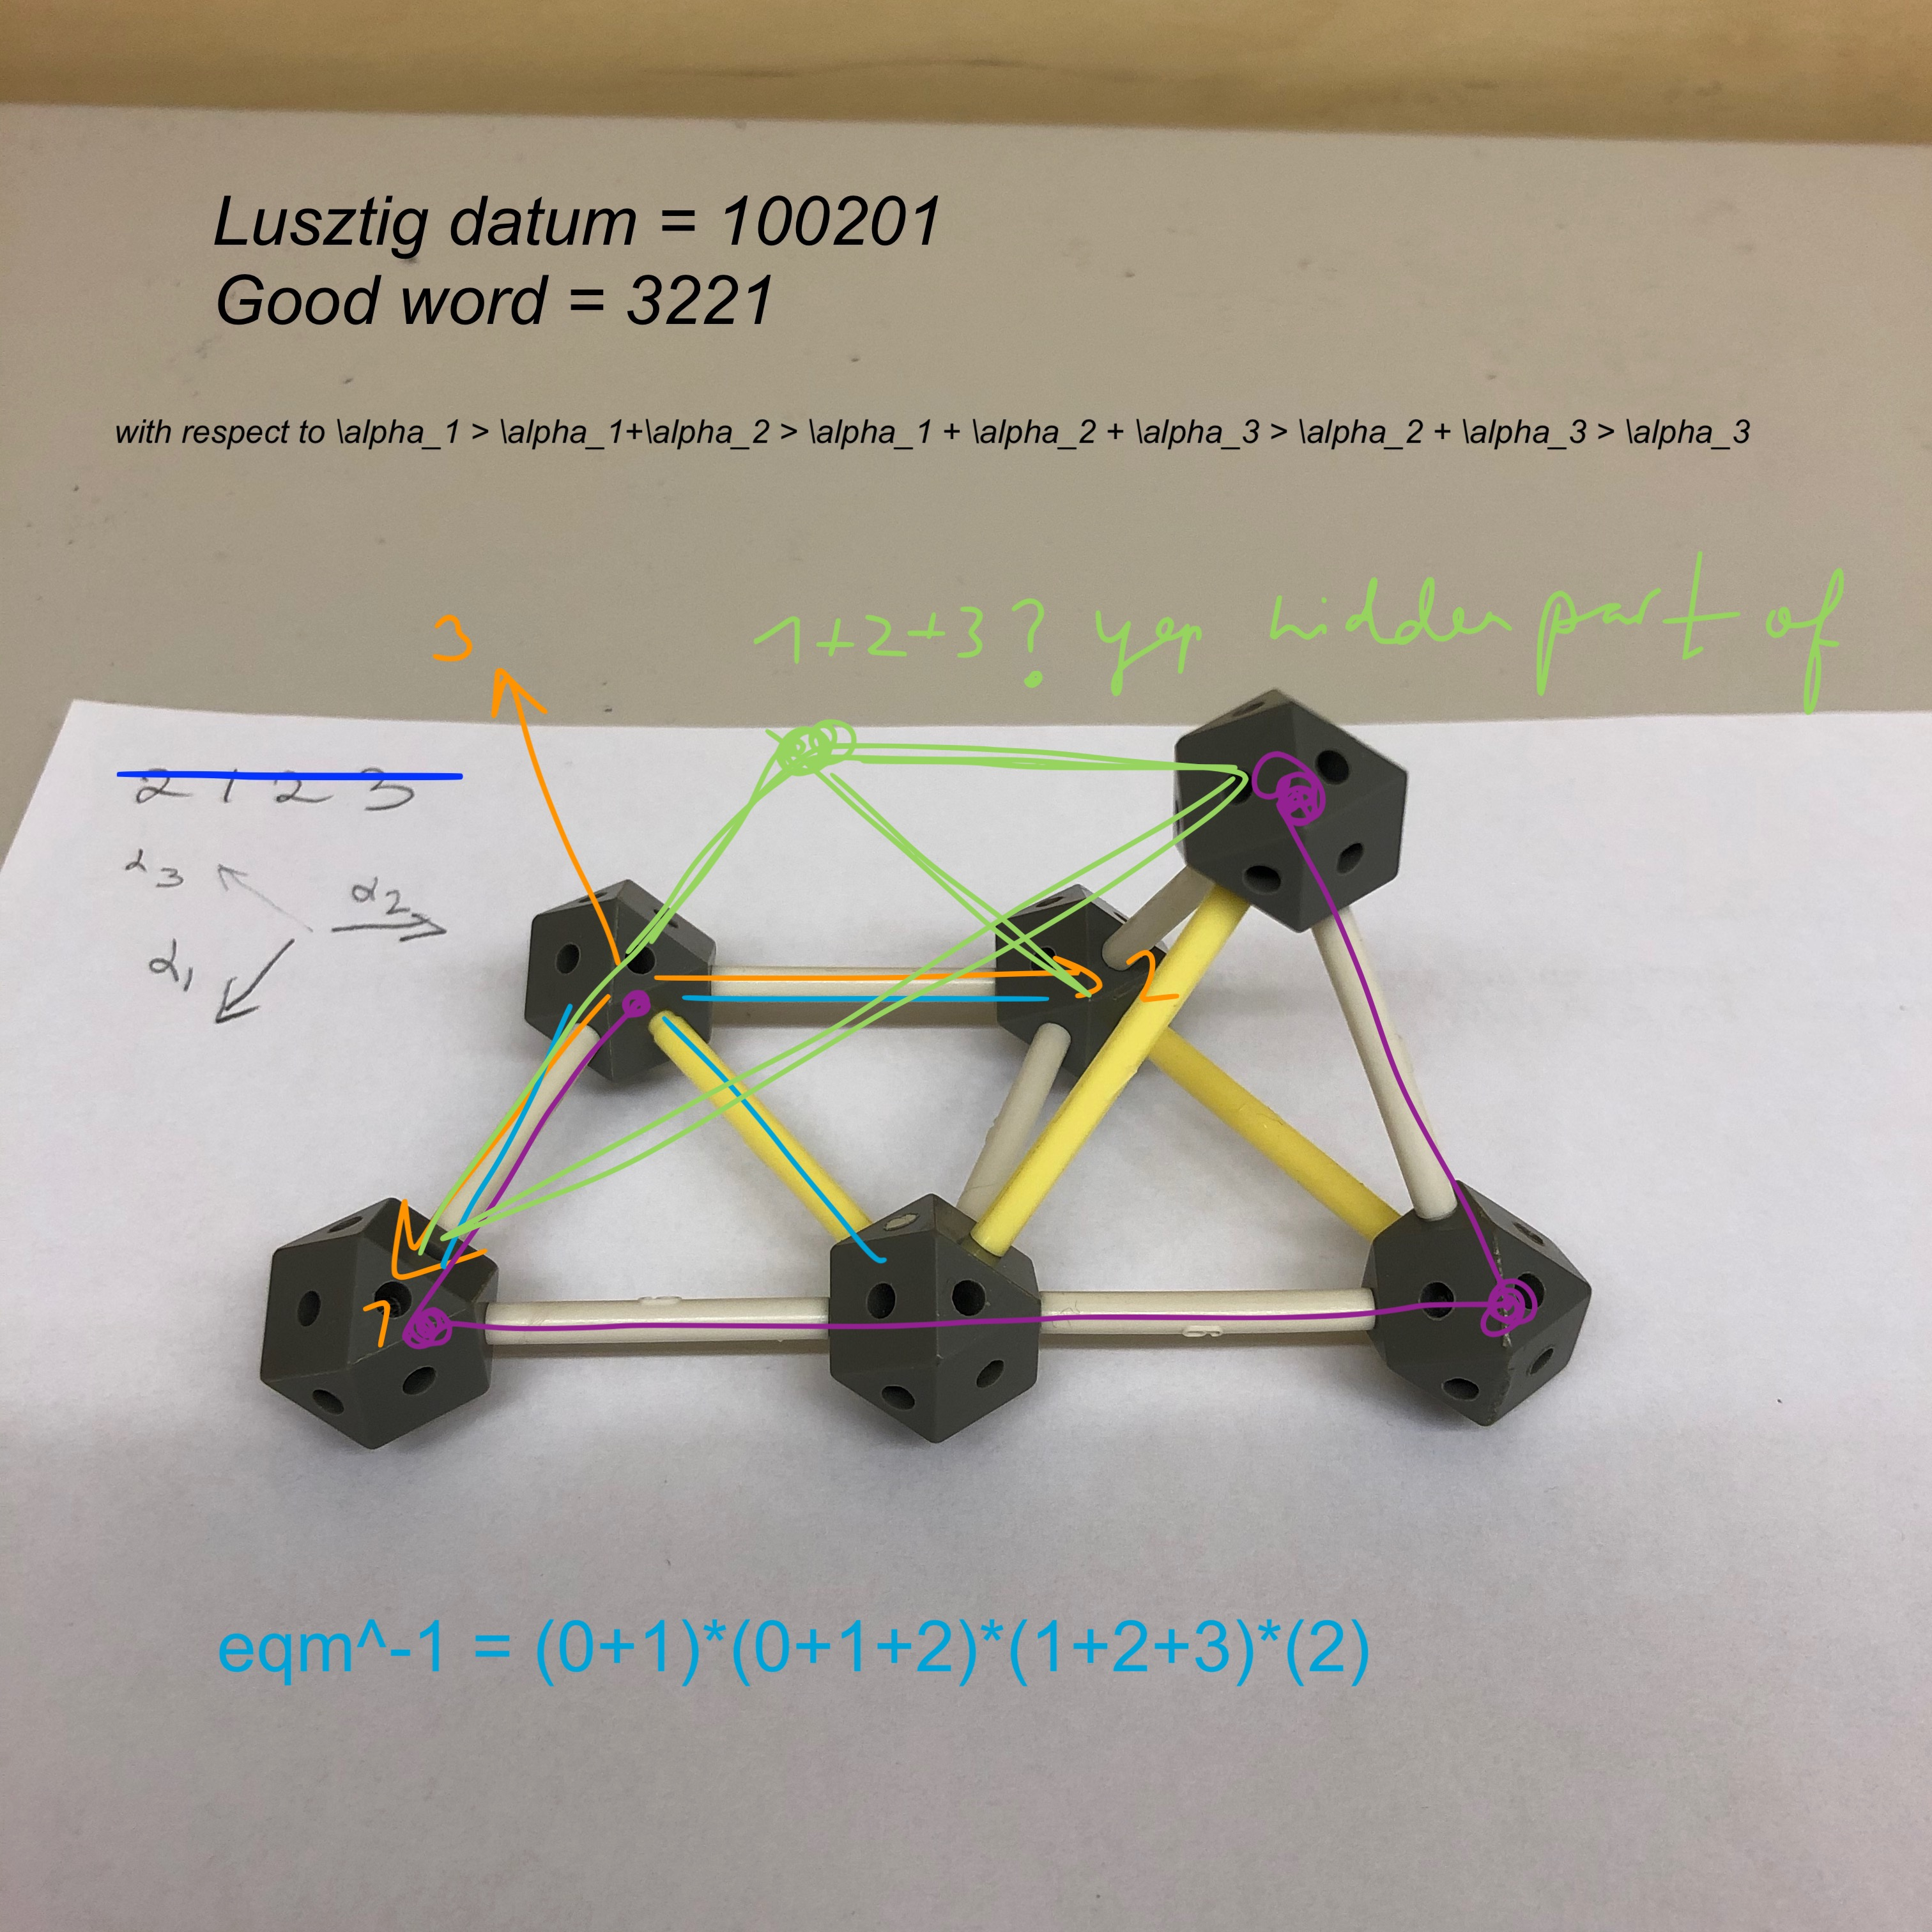
\includegraphics[height=100px]{img/3221.jpeg}
\end{gathered} = \Conv(1, 1 + 2, 1 + 2 + 2, 1 + 2 + 3, 2, \nu) 
\]
% 
From its tableau 
$$\young(112,233,4)$$
we find the ideal of the corresponding MV cycle in $\CC[a_1..a_9]$ by imposing rank conditions on matrices of the form below (left) 
$$\begin{pmatrix}
    0&1&0&0&0&0&0\\
    0&0&{a}_{1}&{a}_{2}&{a}_{3}&{a}_{4}&{a}_{5}\\
    0&0&0&1&0&0&0\\
    0&0&0&0&{a}_{6}&{a}_{7}&{a}_{8}\\
    0&0&0&0&0&1&0\\
    0&0&0&0&0&0&{a}_{9}\\
    0&0&0&0&0&0&0\end{pmatrix} \mapsto \begin{pmatrix}
        t^2 & \\
        - a_1 - a_2 t & t^2 \\
        -a_3 -a_4 t & -a_6 - a_7t & t^2 \\
        - a_5 & -a_8 & -a_9 & t
\end{pmatrix}
$$
coming from the shapes of the nested sequence of subtableaux of $\tau$ 
$$
\young(11,2) \subset \young(112,2) \subset \young(112,23) \subset \young(112,233)
$$
so $I = \left({a}_{1},{a}_{3},{a}_{6},{a}_{8},{a}_{9}\right)$. 
Note that $w(\tau) = {123\atop 132}$ and the first entry in the last column of the matrix above is free.
Its multidegree is
% \todo{is} 
$$
\mdeg I 
% = \alpha_1(\alpha_1 + \hbar)(\alpha_1 + \alpha_2)(\alpha_2)(\alpha_3)
= (\alpha_1) (\alpha_1 + \alpha_2) (\alpha_2) (\alpha_2 + \alpha_3) (\alpha_3)
$$ 
So its equivariant multiplicity (at zero) is 
$$
\varepsilon^{T\times\CC^\times}_0(I) = 
% \frac{1}{(\alpha_1 + \alpha_2 + \hbar)(\alpha_1 + \alpha_2 + \alpha_3)(\alpha_2 + \hbar)(\alpha_2 + \alpha_3)}
\frac 1 {(\alpha_1 + \hbar)(\alpha_1 + \alpha_2 + \hbar) (\alpha_1 + \alpha_2 + \alpha_3)(\alpha_2 + \hbar)}
$$
Using M2 we find that $I$ has Hilbert series
\[
    \frac{1}{\left(1-{T}_{0}{T}_{1}{T}_{2}\right)\left(1-{T}_{0}{T}_{1}{T}_{3}\right)\left(1-{T}_{1}{T}_{3}\right)\left(1-{T}_{0}{T}_{3}\right)}
\]
Using JB, the character of the corresponding simple $L$ is 
% IC[5] =
\[
    \ch L = [2|3|2|1]+[3|2|1|2]+(q+q^{-1})[3|2|2|1]
\]
So 
{\small 
\[
    \barD(L) = \frac{\left({a}_{1}{a}_{2}q^{2}+{a}_{2}^{2}q^{2}+{a}_{2}{a}_{3}q^{2}+{a}_{1}^{2}q+2\,{a}_{1}{a}_{2}q+2\,{a}_{2}^{2}q+{a}_{1}{a}_{3}q+{a}_{1}{a}_{2}+{a}_{2}^{2}+{a}_{2}{a}_{3}\right)}{\left(q\right)\left({a}_{2}\right)\left({a}_{1}\right)\left({a}_{1}+{a}_{2}\right)\left({a}_{1}+{a}_{2}+{a}_{
    3}\right)\left({a}_{1}+2\,{a}_{2}\right)\left({a}_{1}+2\,{a}_{2}+{a}_{3}\right)}
\]}
and evaluating at $q = 1$ we recover
\[
    \frac{1}{\left({a}_{2}\right)\left({a}_{1}\right)\left({a}_{1}+{a}_{2}\right)\left({a}_{1}+{a}_{2}+{a}_{3}\right)}    
\]
\end{description}
% 
\section*{Takeaways?}
Elie? Joel? Todo.. 
\joel{One think that came to my mind from these examples is the following:
Essentially the problem is to try to guess how to go from Elie's
$\barD_q$ and your $T \times \CC^\times$-equivariant multiplicity. So we need
to figure out how to convert between the $q$ and the $\hbar$.  The
simplest situation is to look for where there is no $q$ and where there
is no $\hbar$.  It seems that the KLR modules without the $q$ are
precisely the ``homogeneous'' ones.  We know that some of these
correspond to Schubert varieties, but not all.  On the other hand,
what are the MV cycles where the $\hbar$ does not appear in the
equivariant multiplicity. From your computations, it seems that these
are the ones where we have a very simple choice of $\mu$ (like all 1s)
for the MVy isomorphism. Is this true? Can these be related to each?

What about simpler examples, in A1 or A2?}

\section*{Smaller examples}
% 
\subsection*{Type $A_1$}
$\nu = n\alpha = \underbrace{(\alpha)+\cdots+(\alpha)}_{n}$ and $n_\bullet = (n)$. There is just one partition for each $\nu$, and hence just one MV cycle. 
\[
\underline{w}[n_\bullet] = 1.1\dots 1\qquad \lambda = (2n)\ge \mu = (n,n)    
\]
The MV polytope will just be the line segment $[0,n]$ in $\RR\alpha$. The tableau will be 
\[
\young(11\tinydots122\tinydots 2)    
\]
The ideal of the corresponding MV cycle in $\CC[a_1..a_n]$ is got by imposing the vacuous condition $A^{2n} = 0$ on 
\[
    A = \left[\begin{BMAT}{cccc:cccc}{cccc:cccc}
        0 & 1 & & & & & & \\
          & 0 & 1 & & & & &  \\
              &  & \ddots & 1 & & & & \\
              &  &  & 0  & a_1 & a_2 & \cdots & a_n \\
              &  &  &    & 0 & 1 & & \\
              &  &  &    &  & 0 & 1 & \\ 
              &  &  &    &  &   & \ddots & 1 \\
              &  &  &    &  &   &  & 0 
    \end{BMAT}\right]\mapsto \begin{bmatrix}
        t^n & 0 \\
        -a_1 - a_2 t - \cdots - a_n t^{n-1} & t^n 
    \end{bmatrix}
\]
In other words, the MV cycle is $\AA^n = \spec \CC[a_1..a_n]$. Its multidegree is just 1, while its equivariant multiplicity is
\[
    \varepsilon_0^{T\times\CC^\times}(\AA^n) = \frac{1}{(\alpha)(\alpha + \hbar)\cdots(\alpha + (n-1)\hbar)}
\]
Compare with the corresponding irreducible character 
\[
???     
\]
% \small$$\left[\begin{BMAT}{ccc:cc:cc:c}{ccc:cc:cc:c}
%     0&1&0&0&0&0&0&0\\
%     0&0&1&0&0&0&0&0\\
%     0&0&0&{a}_{1}&{a}_{2}&{a}_{3}&{a}_{4}&{a}_{5}\\
%     0&0&0&0&1&0&0&0\\
%     0&0&0&0&0&{a}_{6}&{a}_{7}&{a}_{8}\\
%     0&0&0&0&0&0&1&0\\
%     0&0&0&0&0&0&0&{a}_{9}\\
%     0&0&0&0&0&0&0&0\end{BMAT}\right]
% 
\subsection*{Type $A_2$}
%
% import bibliography from tex.bib file
%
\bibliographystyle{plain}
\bibliography{tex}
%
% for bundling, bbl file contains
%
% \begin{thebibliography}{E-G-S}

% \bibitem[A1]{Anderson00}
% J.~E.~Anderson, \textit{On Mirkovi\'c and Vilonen's Intersection Homology cycles for the Loop Grassmannian.} PhD thesis, Princeton University, 2000.

% \end{thebibliography}
%
\end{document}